\documentclass[12pt]{article}
\usepackage[utf8]{inputenc}
\usepackage{geometry}
\geometry{a4paper, margin=1in}
\usepackage{graphicx}
\usepackage{hyperref}
\usepackage{booktabs}
\usepackage{float}
\usepackage{parskip}

\begin{document}

\begin{titlepage}
    \centering
    \vspace*{2cm}
    
    {\Large \textbf{Machine Learning Assignment} \par}
    \vspace{0.5cm}
    {\large CM4371 - Machine Learning \& Pattern Recognition \par}
    
    \vspace{6cm}
    
    {\Large \textbf{Sri Lanka Property Price Prediction System} \par}
    
    \vspace{1cm}
    {\Large \textbf{Jayatissa P.B.N. -- 214092B} \par}
    
    \vfill
    
    {\large Faculty of Information Technology \par}
    {\large University of Moratuwa \par}
    \vspace{0.5cm}
    {\large 2026 \par}
\end{titlepage}

\tableofcontents
\newpage

\section{Introduction}
The Sri Lankan real estate market is highly dynamic and diverse, with property prices varying significantly based on location, size, and amenities. Due to the complex interplay of these factors, manually estimating a property's market value can be difficult, subjective, and prone to inaccuracies.

In this project, a machine learning-based system is developed to predict property prices in Sri Lanka using structured data from online listings. By employing advanced regression techniques on local real-world data and integrating Explainable AI (XAI) methods, the model offers transparent and accurate price estimates. The final system is deployed with a user-friendly web interface that allows prospective buyers and sellers to obtain instant property valuations based on key characteristics.

\section{Problem Definition}
The primary focus of this project is to accurately predict the selling price of residential properties in the Sri Lankan market using machine learning. The goal is to estimate a property's market value based on tangible features such as the number of bedrooms, bathrooms, land size, house size, city, and district.

This is framed as a supervised regression problem, where the target variable is the property price in Sri Lankan Rupees (LKR), and the input variables are the property characteristics. Providing an objective, data-driven pricing model addresses the inconsistencies and subjective biases of manual valuations, helping buyers make informed decisions and sellers price their properties competitively.

\section{Dataset Collection and Preprocessing}
The dataset used for this study was collected from \texttt{ikman.lk}, a popular Sri Lankan online marketplace, using web scraping techniques. The raw dataset consisted of 15,327 property listings representing real-world advertisements across various districts.

Each record contained the following initial features:
\begin{itemize}
    \item Bedrooms
    \item Bathrooms
    \item Land Size (in perches)
    \item House Size (in sqft)
    \item Location (City and District)
    \item Price (Target Variable in LKR)
\end{itemize}

To ensure high data quality and model reliability, several preprocessing steps were undertaken:
\begin{itemize}
    \item \textbf{Data Parsing:} Text-based strings (e.g., ``Rs 5,400,000'', ``50.0 perches'', ``10+ beds'') were parsed into standardized numeric formats.
    \item \textbf{Location Extraction:} The raw location string was split into distinct categorical features: \texttt{City} and \texttt{District}.
    \item \textbf{Handling Missing Values:} Rows representing incomplete listings or missing target prices (zero/NaN) were removed.
    \item \textbf{Outlier Removal:} Extreme price anomalies outside the 1st and 99th percentiles were filtered out. Unrealistic land sizes ($>500$ perches) and house sizes ($>20,000$ sqft) were also removed, along with ensuring bedrooms and bathrooms stayed within realistic ranges.
\end{itemize}

After preprocessing, the final cleaned dataset consisted of \textbf{15,003 high-quality records}. No personal or sensitive seller information was retained.

\section{Exploratory Data Analysis}
Exploratory Data Analysis (EDA) was conducted to uncover the underlying distribution of property prices and the correlation between the features.

Key findings included:
\begin{itemize}
    \item \textbf{Price Distribution:} The property prices demonstrated a right-skewed distribution, highlighting the presence of high-value luxury real estate within the market. This skewness suggests non-linear relationships between property characteristics and their valuation.
    \item \textbf{Feature Correlations:} \texttt{House Size} and \texttt{Land Size} established strong positive correlations with the property price, while the number of \texttt{Bedrooms} and \texttt{Bathrooms} also exhibited positive, albeit slightly weaker, relationships.
    \item \textbf{Locational Influence:} Categorical variables like \texttt{City} and \texttt{District} were found to heavily influence property values, indicating a significant location premium in real estate pricing.
\end{itemize}

The complexity of these relationships strongly indicated that tree-based ensemble methods would outperform simple linear models.

\section{Algorithm Selection}
The \textbf{CatBoost Regressor} was selected as the primary machine learning algorithm. CatBoost is an advanced gradient boosting decision tree algorithm uniquely designed to manage categorical features natively and prevent overfitting.

Reasons for selecting CatBoost included:
\begin{itemize}
    \item \textbf{Native Categorical Handling:} The dataset consists of high-cardinality categorical features such as \texttt{City} and \texttt{District}. CatBoost efficiently encodes these features internally without the need for manual one-hot encoding, saving memory and processing time.
    \item \textbf{Handling Non-linear Relationships:} As observed during EDA, the relationship between property attributes and price is highly non-linear. CatBoost captures these complex interactions exceptionally well.
    \item \textbf{Robustness:} It handles outliers gracefully and minimizes overfitting compared to standalone decision trees or traditional regression models.
\end{itemize}

\section{Model Training and Evaluation}

\subsection{Train--Test Split}
The cleaned dataset of 15,003 records was divided randomly into a training set (80\%) and a testing set (20\%). The model was fit on the training data, while the testing data evaluated its real-world generalization potential.

\subsection{Hyperparameter Selection}
The CatBoost Regressor was configured with the following key hyperparameters to balance complexity and runtime efficiency:
\begin{itemize}
    \item \textbf{Iterations:} 1000
    \item \textbf{Learning rate:} 0.05
    \item \textbf{Tree depth:} 8
    \item \textbf{L2 Leaf Regularization:} 3
    \item \textbf{Loss function:} RMSE
    \item \textbf{Early Stopping:} 50 rounds (to halt training automatically if validation performance plateaued)
\end{itemize}

\subsection{Performance Metrics \& Results}
The regression model achieved the following performance metrics on the unseen test set:

\begin{table}[H]
    \centering
    \begin{tabular}{@{}ll@{}}
        \toprule
        \textbf{Metric} & \textbf{Value} \\ \midrule
        Mean Absolute Error (MAE) & 5.68 Million LKR \\
        Root Mean Squared Error (RMSE) & 11.72 Million LKR \\
        R\textsuperscript{2} Score & \textbf{0.8415} \\ \bottomrule
    \end{tabular}
    \caption{Model Performance on Test Set}
\end{table}

The robust R\textsuperscript{2} score of $\sim$0.84 indicates that the model successfully explains over 84\% of the variance in Sri Lankan property prices. Given the vast range of property values (from basic homes to luxury multi-million-rupee estates), the MAE of 5.68M LKR represents a fair average prediction drift.

\subsection{Model Behavior Analysis}
The actual vs. predicted plot and residual distribution graphs produced during training verified model stability. Residuals were normally distributed around zero, showing that the model does not carry a strong systematic bias and is equally likely to slightly over-predict or under-predict property values based on the learned relationships.

\begin{figure}[H]
    \centering
    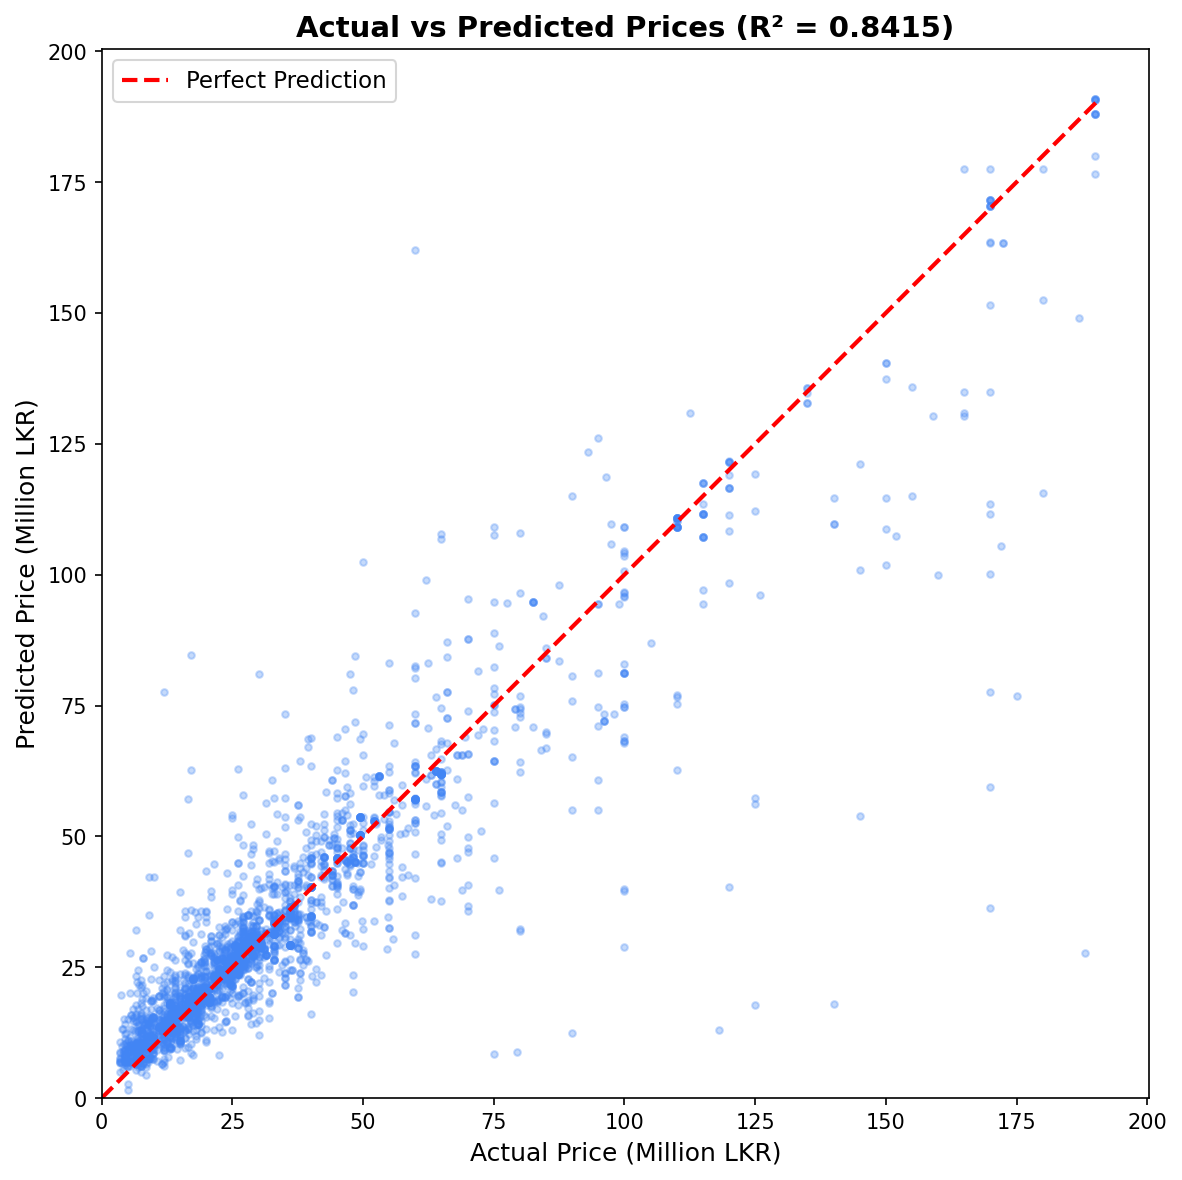
\includegraphics[width=0.48\textwidth]{notebooks/actual_vs_predicted.png}
    \hfill
    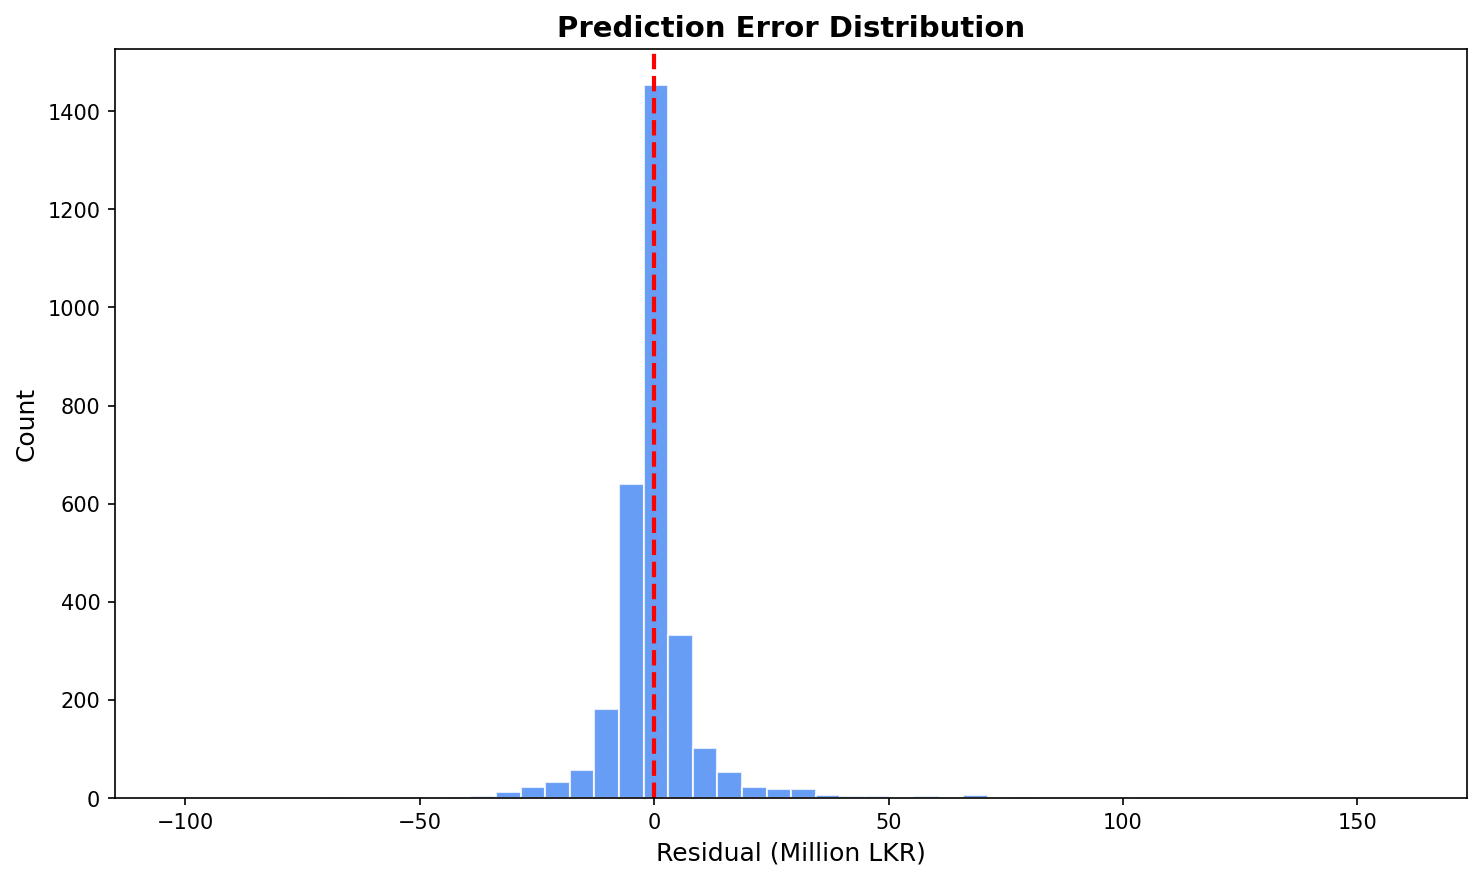
\includegraphics[width=0.48\textwidth]{notebooks/residual_distribution.png}
    \caption{Actual vs. Predicted Prices and Residual Distribution}
\end{figure}

\section{Explainability and Interpretation}
To prevent the model from becoming an opaque ``black-box,'' Explainable AI (XAI) tools were integrated.

\subsection{Feature Importance Analysis}
Using CatBoost's internal feature importance metric, the features contributing most significantly to price determination were identified:
\begin{enumerate}
    \item \textbf{City} (Most influential)
    \item \textbf{House Size (Sqft)}
    \item \textbf{Land Size (Perches)}
    \item \textbf{Bathrooms}
    \item \textbf{Bedrooms}
    \item \textbf{District}
\end{enumerate}

This logically aligns with the well-known real estate adage ``location, location, location,'' followed closely by physical property dimensions.

\begin{figure}[H]
    \centering
    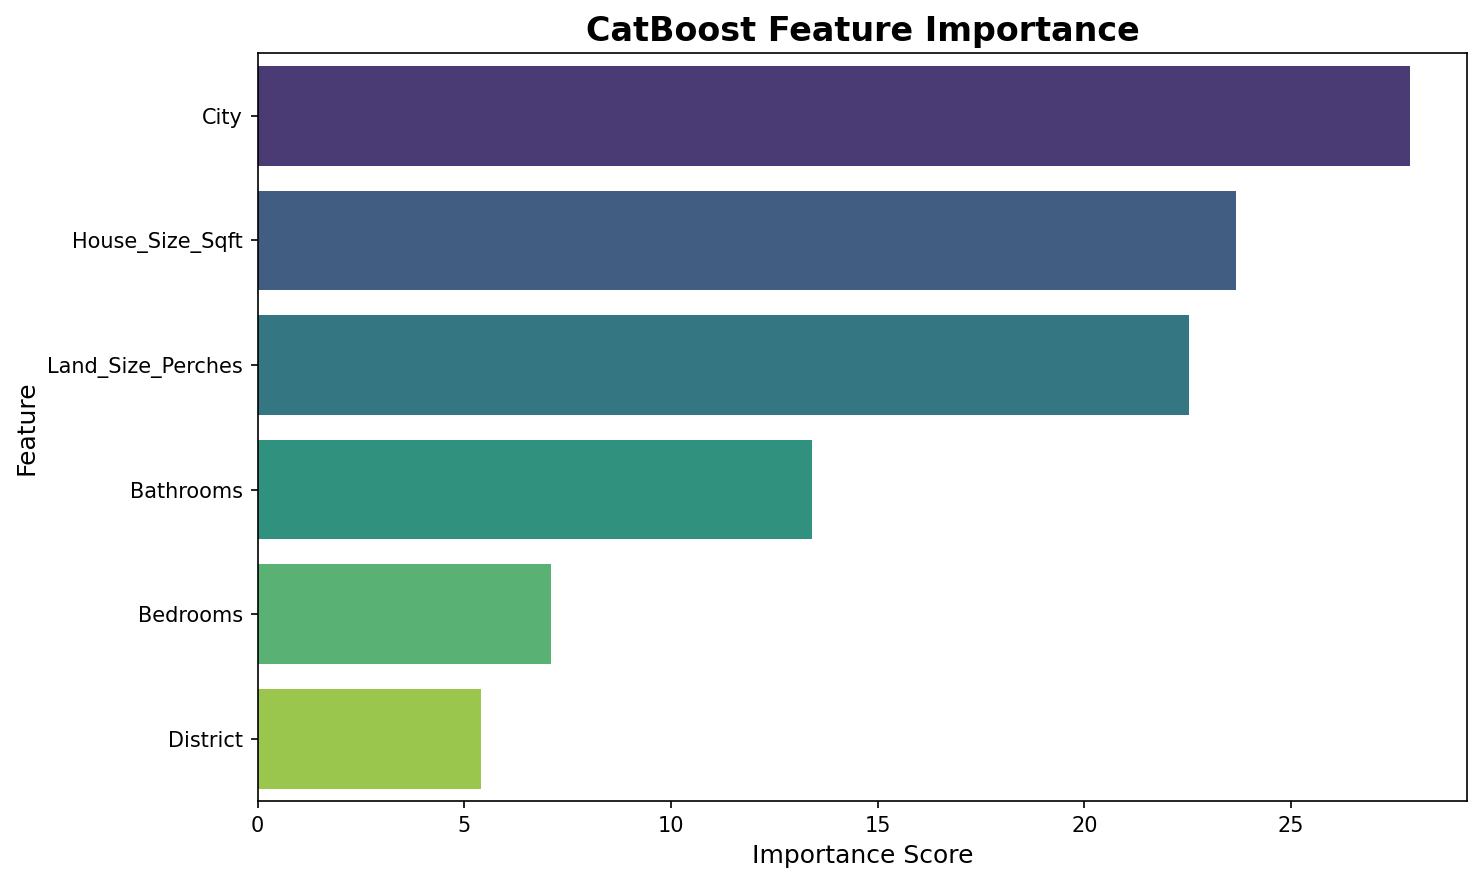
\includegraphics[width=0.8\textwidth]{notebooks/feature_importance.png}
    \caption{CatBoost Feature Importance}
\end{figure}

\subsection{SHAP Analysis}
SHAP (SHapley Additive exPlanations) values provided deeper interpretability:
\begin{itemize}
    \item \textbf{House \& Land Size:} SHAP summary plots confirmed that larger properties consistently push predicted prices higher.
    \item \textbf{City:} Location drove the largest variance in SHAP values, confirming that properties in highly-demanded cities like Colombo carry massive price premiums compared to properties of identical size in less-demanded regions.
\end{itemize}

\begin{figure}[H]
    \centering
    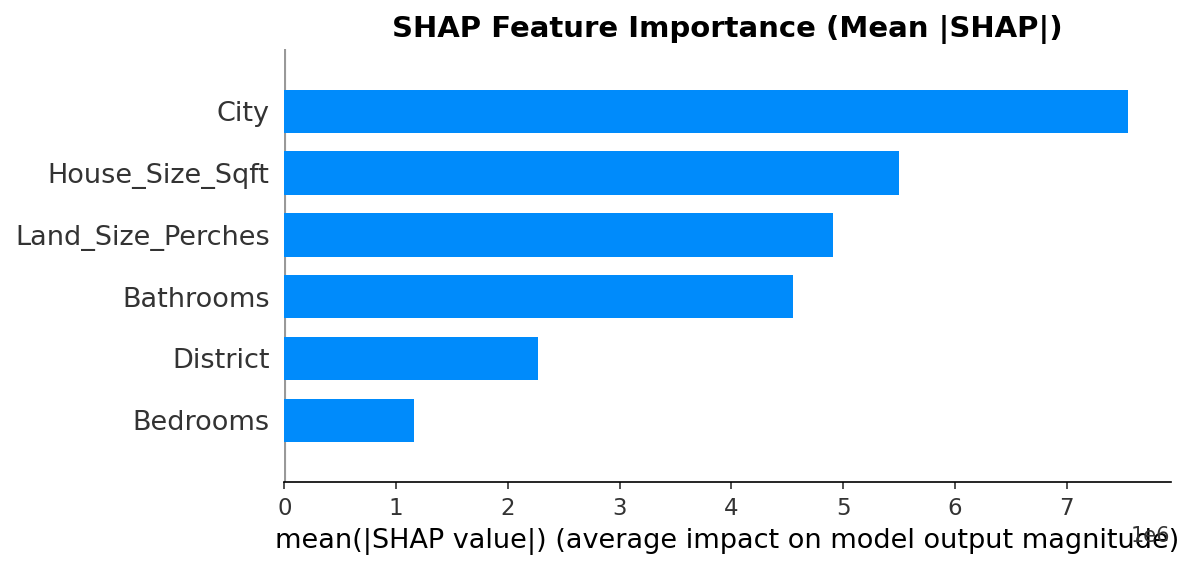
\includegraphics[width=0.8\textwidth]{notebooks/shap_bar.png}
    \caption{SHAP Feature Importance (Mean |SHAP|)}
\end{figure}

\begin{figure}[H]
    \centering
    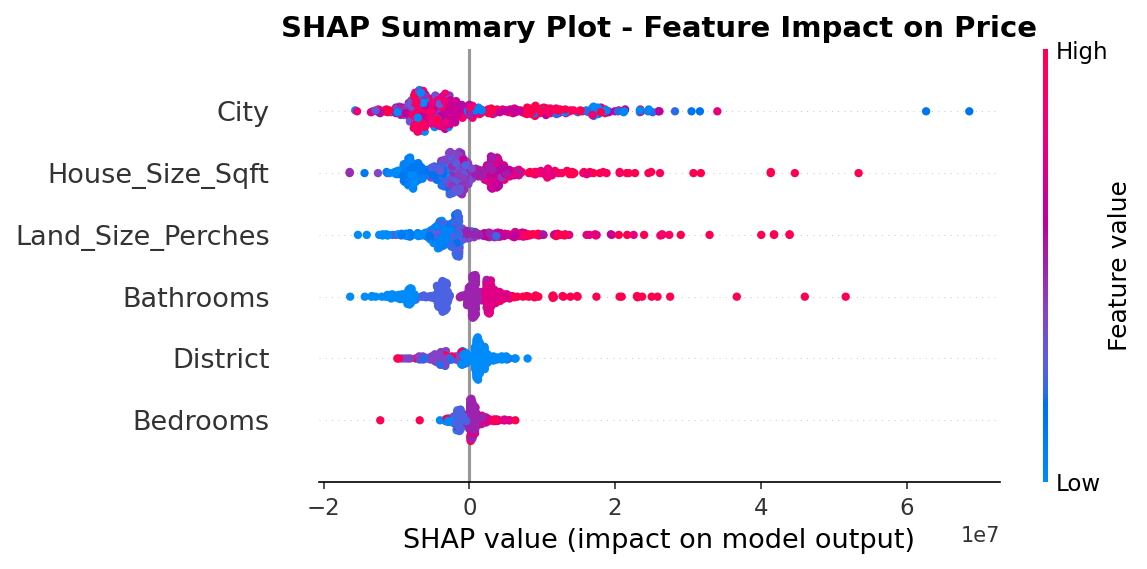
\includegraphics[width=0.8\textwidth]{notebooks/shap_summary.png}
    \caption{SHAP Summary Plot}
\end{figure}

\section{Front-End Integration and Deployment}
To make the predictive power accessible, the model was integrated into a full-stack web application.
\begin{itemize}
    \item \textbf{Backend (FastAPI):} A high-performance Python backend loads the serialized model (\texttt{catboost\_model.pkl}) and exposes a \texttt{/predict} API endpoint.
    \item \textbf{Frontend (HTML/JS/CSS):} A visually appealing, responsive web interface allows users to select a district, specify a city, and input basic property parameters. User interactions trigger asynchronous requests to the backend, rendering real-time price predictions on-screen.
    \item \textbf{Deployment Strategy:} Both services were containerized via \textbf{Docker} and managed completely using \texttt{docker-compose}, guaranteeing consistent cross-platform execution.
\end{itemize}

\section{Critical Discussion}

\subsection{Limitations of the Model}
While robust, the model generates predictions based purely on listing prices, representing sellers' \textit{asking} prices rather than finalized transaction prices. Actual sale values are typically lower post-negotiation. Moreover, the model lacks access to granular details such as architectural quality, internal furnishings, exact neighborhood prestige, and proximity to infrastructure, which undoubtedly sway property value.

\subsection{Data Quality Issues}
Web-scraped data inherently possesses noise. Despite rigorous data cleaning, certain user-entered listings may contain exaggerated land sizes or placeholder prices that slipped through outlier constraints.

\subsection{Risk of Bias and Unfairness}
The model relies entirely on historical marketplace data, meaning it naturally replicates current housing trends. High-income areas with inflated listing prices maintain higher predicted baselines. It runs the risk of perpetuating historic geographic inequalities by reinforcing high prices in currently favored neighborhoods.

\subsection{Real-World Impact and Ethical Considerations}
This system effectively democratizes access to real estate insights, functioning as a fast, data-backed consultant for average buyers who otherwise rely on biased human brokers. Ethically, no personally identifiable information (PII) of property owners was stored or utilized. However, predictions must be contextualized as estimations rather than absolute financial truths, and the application serves purely a decision-support role in the Sri Lankan real estate ecosystem.

\end{document}
